\chapter{City Geometry}
\begin{quote} 
I always like a good math solution to any love problem.

\hfill---Carrie Bradshaw
%You talkin' to me? You talkin' to me? You talkin' to me?
%
%\hfill---Travis Bickle
%
%Thank you very much! 
%\hfill---Latka Gravas
\end{quote}



\section{Welcome to the City}\marginnote{The approach taken in this section was adapted from \cite{krause}.}


One day I was walking through the city---that's right, New York City. I
had the most terrible feeling that I was lost. I had just passed a
\textit{Starbucks Coffee} on my left and a \textit{Sbarro Pizza} on my
right, when what did I see? Another \textit{Starbucks Coffee} and
\textit{Sbarro Pizza}! Three options occurred to me:
\begin{enumerate}
\item I was walking in circles.
\item I was at the nexus of the universe.\index{nexus of the universe}
\item New York City had way too many \textit{Starbucks} and \textit{Sbarro Pizzas}!
\end{enumerate}
Regardless, I was lost. My buddy Joe came to my rescue. He pointed out that the city is organized like a grid. 

``Ah! city geometry!'' I exclaimed.\index{city geometry}\index{geometry!City} At this point all Joe could say was
``Huh?''


\begin{question} What the heck was I talking about?
\end{question}

Let me tell you: \textit{Euclidean geometry}\index{geometry!Euclidean}
is regular old plane (not plain!) geometry. It is the geometry that
we've been exploring thus far in our journey.  In \textit{city
  geometry} we have points and lines, just like in Euclidean geometry.
However, most cities can be viewed as a grid of city blocks
\[
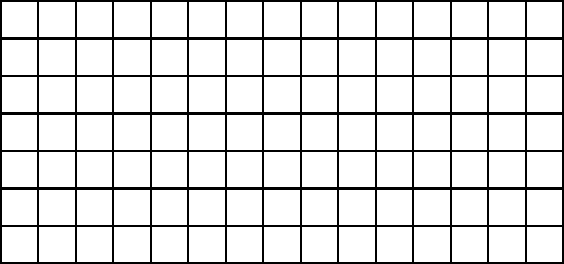
\includegraphics{../graphics/citygrid.pdf}
\]
and when we travel in a city, we can only travel on the streets---we
can't cut through the blocks. This means that we don't measure
distance as the crow flies. Instead we use the \textit{taxicab
  distance}:

\begin{definition}\index{taxicab distance}\index{d@$d$!taxicab}\index{distance!taxicab}Given two points $A = (a_x,a_y)$ and $B = (b_x,b_y)$, we define the
\textbf{taxicab distance} as:
\[
d_T(A,B) = |a_x - b_x| + |a_y - b_y|
\]
\end{definition}


\begin{example} Consider the following points:
\[
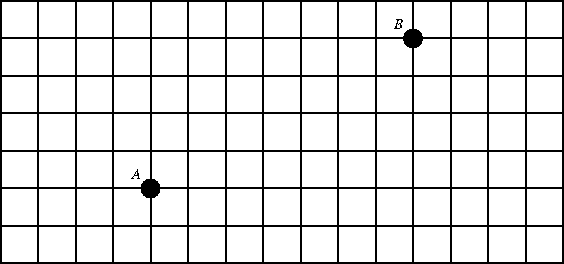
\includegraphics{../graphics/citygrideg1.pdf}
\]
Let $A = (0,0)$. Now we see that $B = (7,4)$. Hence
\begin{align*}
d_T(A,B) &= |0 - 7| + |0-4|\\
&= 7 + 4 \\
&= 11.
\end{align*}
Of course in real life, you would want to add in the appropriate units
to your final answer.
\end{example}

\begin{question} How do you compute the distance between $A$ and $B$ as the crow flies?
\end{question}
\QM

\begin{definition}\index{city geometry}\index{geometry!city}
The geometry where points and lines are those from Euclidean geometry
but distance is measured via taxicab distance is called \textbf{city
  geometry}.
\end{definition}

\begin{question} Compare and contrast the notion of a line in Euclidean geometry and in city geometry. In either geometry is a line the unique shortest path between any two points?
\end{question}
\QM



\subsection{(Un)Common Structures}

How different is life in city geometry from life in Euclidean
geometry? Let's find out!

\subsubsection{Triangles}

If we think back to Euclidean geometry, we
may recall some lengthy discussions on triangles. Yet so far, we have
not really discussed triangles in city geometry.

\begin{question} What does a triangle look like in city geometry and how do you measure its angles? \index{city geometry!triangle}\index{triangle!city geometry}
\end{question}

I'll take this one. Triangles look the same in city geometry as they
do in Euclidean geometry. Also, you measure angles in exactly the same
way. However, there is one minor hiccup. Consider these two triangles
in city geometry:
\[
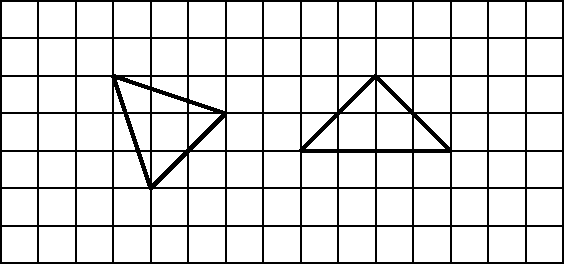
\includegraphics{../graphics/citytri.pdf}
\]
\begin{question} 
What are the lengths of the sides of each of these triangles? Why is
this odd?
\end{question}
\QM 

Hence we see that triangles are a bit funny in city geometry.

\subsubsection{Circles}

Circles are also discussed in many geometry courses and this course is
no different. However, in city geometry the circles are a little less
round. The first question we must answer is the following:

\begin{question} What is a circle?
\end{question}

Well, a circle is the collection of all points equidistant from a
given point. So in city geometry, we must conclude that a circle of
radius $2$ would look like:
\[
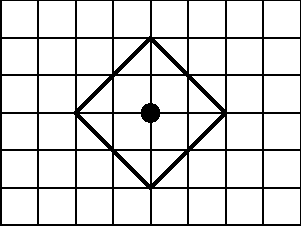
\includegraphics{../graphics/citycircle.pdf}
\]
\index{circle!city geometry}\index{city geometry!circle}
\begin{question} What sort of shape should a city geometry compass draw?
\end{question}
\QM

\begin{question} 
How many points are there at the intersection of two circles in
Euclidean geometry? How many points are there at the intersection of
two circles in city geometry?
\end{question}
\QM


\begin{problems}
\begin{enumerate}
\item Given two points $A$ and $B$ in city geometry, does $d_T(A,B) =
  d_T(B,A)$? Explain your reasoning.
\item It was once believed that Euclid's five postulates
\begin{enumerate}
\item A line can be drawn from a point to any other point.
\item A finite line can be extended indefinitely.
\item A circle can be drawn, given a center and a radius.
\item All right angles are ninety degrees. 
\item If a line intersects two other lines such that the sum of the
  interior angles on one side of the intersecting line is less than
  the sum of two right angles, then the lines meet on that side and
  not on the other side.
\end{enumerate}
were sufficient to completely describe plane geometry.  Explain how
city geometry shows that Euclid's five postulates are \textbf{not}
enough to determine all of the familiar properties of the plane.

\item In Euclidean geometry are all equilateral triangles congruent
  assuming they have the same side length? Is this true in city
  geometry? Explain your reasoning.

\item How many points are there at the intersection of two circles in
  Euclidean geometry? How many points are there at the intersection of
  two circles in city geometry? Explain your reasoning.

\item What sort of shape should a city geometry compass draw? Explain
  your reasoning.

\item Give a detailed discussion of what happens if we attempt the
  compass and straightedge construction for an equilateral triangle
  using a city geometry compass.

\item Give a detailed discussion of what happens if we attempt the
  compass and straightedge construction for bisecting a segment using
  a city geometry compass.

\item Give a detailed discussion of what happens if we attempt the
  compass and straightedge construction for a perpendicular through a
  point using a city geometry compass.

\item Give a detailed discussion of what happens if we attempt the
  compass and straightedge construction for bisecting an angle using a
  city geometry compass.

\item Give a detailed discussion of what happens if we attempt the
  compass and straightedge construction for copying an angle using a
  city geometry compass.

\item Give a detailed discussion of what happens if we attempt the
  compass and straightedge construction for a parallel through a point
  using a city geometry compass.
\end{enumerate}
\end{problems}

\newpage


\section{Anatomy of Figures and the City}

When we study geometry, what do we seek? That's right---we wish to
discover the points that can be obtained given a set of rules. With
city geometry, the major rule involved is the taxicab distance. Let's
answer these questions!

\begin{question} 
In regards to city geometry, what is a \textit{point}?
\end{question}
\QM

\begin{question}
In regards to city geometry, what is a \textit{line}?
\end{question}
\QM


\begin{question}
In regards to city geometry, what is a \textit{circle}?
\end{question}
\QM


Now I'm going to quiz you about them (I know we've already gone over
this \textit{twice}, but it is fundamental so just smile and answer
the questions):

\begin{question} 
Place two points randomly in the plane. Do you expect to be able to
draw a single line that connects them?
\end{question}
\QM

\begin{question} 
Place three points randomly in the plane. Do you expect to be able to
draw a single line that connects them?
\end{question}
\QM

\begin{question} 
Place two lines randomly in the plane. How many points do you expect
them to share?
\end{question}
\QM


\begin{question} 
Place three lines randomly in the plane. How many points do you expect
all three lines to share?
\end{question}
\QM

\begin{question} 
Place three points randomly in the plane. Will you (almost!) always be
able to draw a city geometry circle containing these points? If no,
why not? If yes, how do you know?
\end{question}
\QM



\subsubsection{Midsets}



\index{city geometry!midset}\index{midset!city geometry}
\begin{definition}
Given two points $A$ and $B$, their \textbf{midset} is the set of points that are an equal distance away from both $A$ and $B$.
\end{definition}
\begin{question}
How do we find the midset of two points in Euclidean geometry? How do we find the midset of two points in city geometry?
\end{question}
In Euclidean geometry, we just take the the following line:
\[
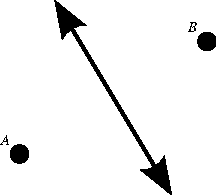
\includegraphics{../graphics/emidset.pdf}
\]
If we had no idea what the midset should look like in Euclidean
geometry, we could start as follows:
\begin{itemize}
\item Draw circles of radius $r_1$ centered at both $A$ and $B$. If these
circles intersect, then their points of intersection will be in our
midset. (Why?)

\item Draw circles of radius $r_2$ centered at both $A$ and $B$. If these
circles intersect, then their points of intersection will be in our
midset.

\item We continue in this fashion until we have a clear idea of what the
midset looks like. It is now easy to check that the line in our
picture is indeed the midset.
\end{itemize}

How do we do it in city geometry? We do it basically the same way.

\begin{example} Suppose you wished to find the midset of two points in city geometry.

We start by fixing coordinate axes. Considering the diagram below, if
$A=(0,0)$, then $B=(5,3)$. We now use the same idea as in Euclidean
geometry. Drawing circles of radius $3$ centered at $A$ and $B$
respectively, we see that there are no points $3$ points away from
both $A$ and $B$. Since $d_T(A,B)=8$, this is to be expected. We will
need to draw larger taxicab circles before we will find points in the
midset. Drawing taxicab circles of radius $5$, we see that the points
$(1,4)$ and $(4,-1)$ are both in our midset.
\[
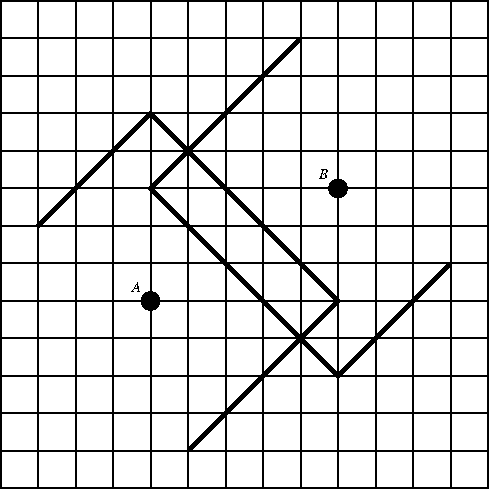
\includegraphics{../graphics/cmidset.pdf}
\]
Now it is time to sing along. You draw circles of radius $6$, to get
two more points $(1,5)$ and $(4,-2)$. Drawing circles with larger
radii yields more and more points ``due north'' of $(1,5)$ and ``due
south'' of $(4,-2)$. However, if we draw circles of radius $4$
centered at $A$ and $B$ respectively, their intersection is the line
segment between $(1,3)$ and $(4,0)$. Unlike Euclidean circles,
distinct city geometry circles can intersect in more than two points and
city geometry midsets can be more complicated than their Euclidean
counterparts. 
\end{example}

\begin{question}How do you draw the city geometry midset of $A$ and
$B$? What could the midsets look like?
\end{question}
\QM






\subsubsection{Parabolas}


Recall that a parabola is a set of points such that each of those
points is the same distance from a given point, $F$, as it is from a
given line, $D$. 
\[
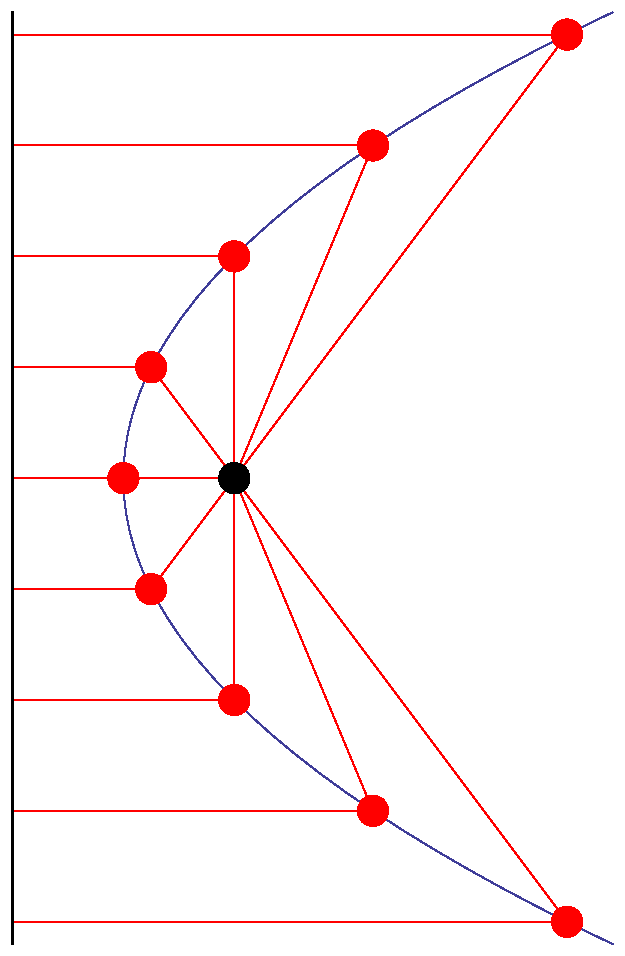
\includegraphics[angle=90,scale=.4]{../graphics/parabolapointline.pdf}
\]
This definition still makes sense when we work with taxicab distance
instead of Euclidean distance. To start, choose a value $r$ and draw a
line parallel to $D$ at taxicab distance $r$ away from $D$. Now draw a
City circle of radius $r$ centered at $F$. The points of intersection
of this line and this circle will be $r$ away from $D$ and $r$ away
from $F$ and so will be points on our City parabola. Repeat this
process for different values of $r$. 
\[
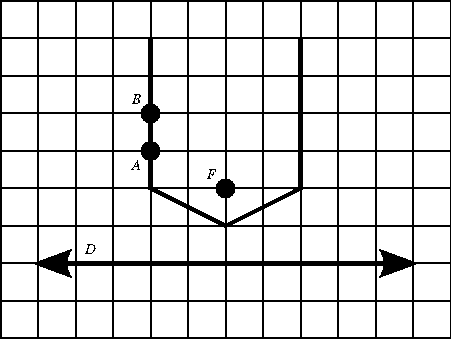
\includegraphics{../graphics/cparabola.pdf}
\]
\index{city geometry!parabola}\index{parabola!city geometry}

Unlike the Euclidean case, the City parabola need not grow broader and
broader as the distance from the line increases. In the picture above,
as we go from $A$ to $B$ on the parabola, both the taxicab and
Euclidean distances to the line $D$ increase by $1$. The taxicab
distance from the point $F$ also increases by $1$ as we go from $A$ to
$B$ but the Euclidean distance increases by less than $1$. For the
Euclidean distance from $F$ to the parabola to keep increasing at the
same rate as the distance to the line $D$, the Euclidean parabola has
to keep spreading to the sides.

\begin{question}How do you draw city geometry parabolas? What do different parabolas look like?
\end{question}
\QM



\subsubsection{A Paradox}

To be completely clear on what a paradox is, here is the definition we
will be using:
\begin{definition}\index{paradox} A \textbf{paradox}\index{paradox} is a statement that seems to be contradictory. This means it seems both true and false at the same time. 
\end{definition}

There are many paradoxes in mathematics. By studying them we gain
insight---and also practice tying our brain into knots! Here is a paradox:

\begin{paradox} $\sqrt{2} = 2$.\index{paradox!$\sqrt{2}=2$}\index{sqrt2@$\sqrt{2}$}
\end{paradox}

\begin{proof}[False-Proof] Consider the following sequence of diagrams:
\[
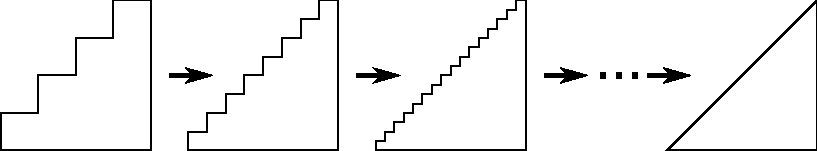
\includegraphics[width=4in]{../graphics/root2para.pdf}
\]
On the far right-hand side, we see a right-triangle. Suppose that the
lengths of the legs of the right-triangle are one. Now by the
Pythagorean Theorem, the length of the hypotenuse is $\sqrt{1^2+1^2}
=\sqrt{2}.$

However, we see that the triangles coming from the left converge to
the triangle on the right. In every case on the left, the stair-step
side has length $2$. Hence when our sequence of stair-step triangles
converges, we see that the hypotenuse of the right-triangle will have
length $2$. Thus $\sqrt{2} = 2$.
\end{proof}

\begin{question} What is wrong with the proof above? 
\end{question}
\QM




\begin{problems}
\begin{enumerate}
\item Suppose that you have two triangles $\triangle ABC$ and $\triangle DEF$ in  city geometry such that
\begin{enumerate}
\item $d_T(A,B) = d_T(D,E)$.
\item $d_T(B,C) = d_T(E,F)$.
\item $d_T(C,A) = d_T(F,D)$.
\end{enumerate} 
Is it necessarily true that $\triangle ABC \equiv \triangle DEF$? Explain your reasoning.
\item In city geometry, if all the angles of $\triangle ABC$ are
  $60^\circ$, is $\triangle ABC$ necessarily an equilateral triangle?
  Explain your reasoning.
\item In city geometry, if two right triangles have legs of the same
  length, is it true that their hypotenuses will be the same length?
  Explain your reasoning.
\item Considering that $\pi$ is the ratio of the circumference of a
  circle to its diameter, what is the value of $\pi$ in city geometry?
  Explain your reasoning.

\item Considering that the area of a circle of radius $r$ is given by
  $\pi r^2$, what is the value of $\pi$ in city geometry? Explain your
  reasoning.

\item When is the Euclidean midset of two points equal to their city
  geometry midset? Explain your reasoning.
\item Find the city geometry midset of $(-2,2)$ and $(3,2)$.
\item Find the city geometry midset of $(-2,2)$ and $(4,-1)$.
\item Find the city geometry midset of $(-2,2)$ and $(2,2)$.
\item Draw the city geometry parabola determined by the point $(0,2)$
  and the line $y=0$.
\item Draw the city geometry parabola determined by the point $(3,0)$
  and the line $x=0$.
\item Draw the city geometry parabola determined by the point $(2,0)$ and
the line $y=x$.
\item Find the distance in city geometry from the point $(3,4)$ to the
  line $y = -1/3x$. Explain your reasoning. 
\item Draw the city geometry parabola determined by the point $(0,4)$
  and the line $y=x/3$. Explain your reasoning. 
\item Draw the city geometry parabola determined by the point $(0,6)$
  and the line $y=x/2$. Explain your reasoning. 
\item Draw the city geometry parabola determined by the point $(1,4)$
  and the line $y=2x/3$. Explain your reasoning. 
\item Draw the city geometry parabola determined by the point $(3,3)$
  and the line $y=x/2$. Explain your reasoning. 
\item Find all points $P$ such that $d_T(P,A)+d_T(P,B)=8$. Explain
  your work. (In Euclidean geometry, this condition determines an
  \textit{ellipse}. The solution to this problem could be called the
  \emph{city geometry ellipse}.)

\item True/False: Three noncollinear points lie on a unique Euclidean
  circle. Explain your reasoning.
\item True/False: Three noncollinear points lie on a unique city geometry
  circle. Explain your reasoning.

\item Explain why no Euclidean circle can contain three collinear
  points. Can a city geometry circle contain three collinear points? Explain
  your conclusion.

\item Can you find a false-proof showing that $\pi = 2$?


\end{enumerate}
\end{problems}

\newpage


\section{Getting Work Done}

If you are interested in \textit{real-world} types of problems, then
maybe city geometry is the geometry for you. The concepts that arise
in city geometry are directly applicable to everyday life.

\begin{question}
Will just bought himself a brand new gorilla suit.\index{gorilla suit}
He wants to show it off at three parties this Saturday night. The
parties are being held at his friends' houses: the
Antidisestablishment $(A)$, Hausdorff $(H)$, and the Wookie Loveshack
$(W)$. If he travels from party $A$ to party $H$ to party $W$, how far
does he travel this Saturday night?
\[
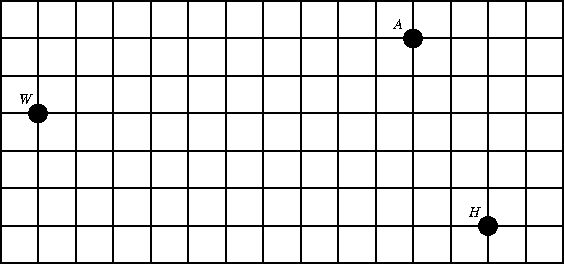
\includegraphics{../graphics/citygrideg2.pdf}
\]
\end{question} 
\begin{proof}[Solution] We need to compute
\[
d_T(A,H)+d_T(H,W)
\]
Let's start by fixing a coordinate system and making $A$ the
origin. Then $H$ is $(2,-5)$ and $W$ is $(-10,-2)$. Then
\begin{align*}
d_T(A,H) &=|0 - 2| + | 0 -(-5)|\\
&= 2+5\\
&=7
\end{align*}
 and 
\begin{align*}
d_T(H,W) &= | 2 - (-10) | + | -5 - (-2)|\\
&= 12 + 3 \\
&= 15.
\end{align*} 
Will must trudge $7+15 = 22$ blocks in his gorilla suit.
\end{proof}



Okay, that's enough monkey business---I feel like pizza and a movie.


\begin{question}
Brad and Melissa are going to downtown Champaign, Illinois. Brad wants
to go to \textit{Jupiter's} for pizza $(J)$ while Melissa goes to
\textit{Boardman's Art Theater} $(B)$ to watch a movie. Where should
they park to minimize the total distance walked by both?
\[
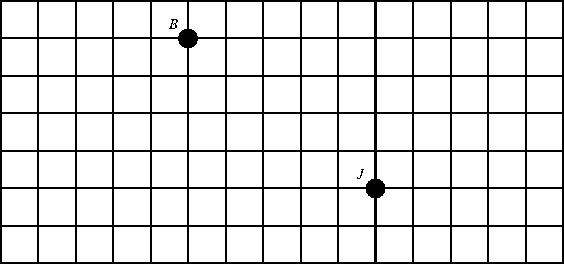
\includegraphics{../graphics/citygrideg3.pdf}
\]
\end{question}

\begin{proof}[Solution]
Again, let's set up a coordinate system so that we can say what points
we are talking about. If $J$ is $(0,0)$, then $B$ is $(-5,4)$.
\[
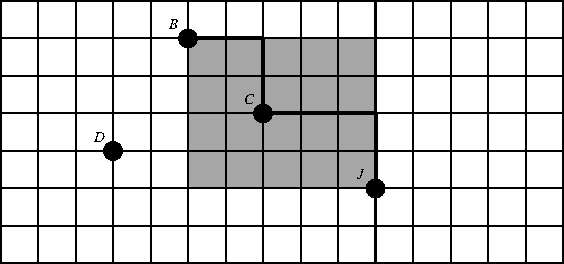
\includegraphics{../graphics/citygrideg4.pdf}
\]
No matter where they park, Brad and Melissa's two paths joined
together must make a path from $B$ to $J$. This combined path has to
be at least $9$ blocks long since $d_T(B,J)=9$. They should look for a
parking spot in the rectangle formed by the points
$(0,0),(0,4),(-5,0)$, and $(-5,4)$.

Suppose they park within this rectangle and call this point
$C$. Melissa now walks $4$ blocks from $C$ to $B$ and Brad walks $5$
blocks from $C$ to $J$. The two paths joined together form a path from
$B$ to $J$ of length $9$.

If they park outside the rectangle described above, for example at
point $D$, then the corresponding path from $B$ to $J$ will be longer
than $9$ blocks. Any path from $B$ to $J$ going through $D$ goes a
block too far west and then has to backtrack a block to the east
making it longer than $9$ blocks.
\end{proof}
\begin{question}
If we consider the same question in Euclidean geometry, what is the
answer?
\end{question}
\QM


\begin{question}
Tom is looking for an apartment that is close to Altgeld Hall $(H)$
but is also close to his favorite restaurant, \textit{Crane
  Alley}\index{Crane Alley} $(C)$. Where should Tom live?
\[
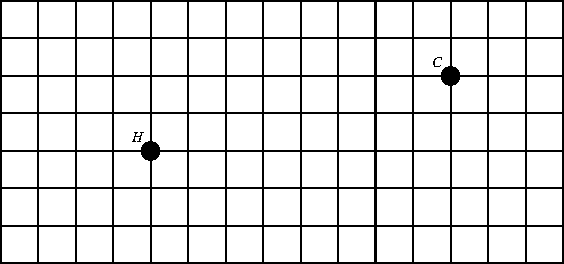
\includegraphics{../graphics/citygrideg6.pdf}
\]
\end{question}
\begin{proof}[Solution]
If we fix a coordinate system with its origin at Altgeld Hall, $H$,
then $C$ is at $(8,2)$. We see that $d_T(H,C)=10$. If Tom wants to
live as close as possible to both of these, he should look for an
apartment, $A$, such that $d_T(A,H)=d_T(A,C)=5$. He would then be
living halfway along one of the shortest paths from Altgeld to the
restaurant. Mark all the points $5$ blocks away from $H$. Now mark all
the points $5$ blocks away from $C$.
\[
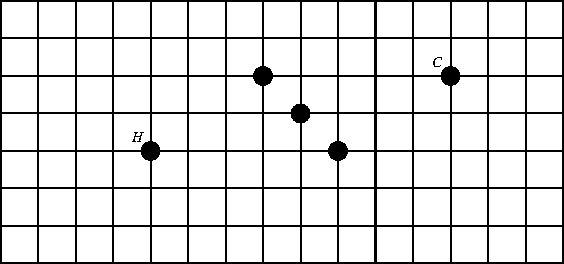
\includegraphics{../graphics/citygrideg7.pdf}
\]
We now see that Tom should check out the apartments near $(5,0), (4,1)$, and $(3,2)$.
\end{proof}



\begin{problems}
\begin{enumerate}
\item Will just bought himself a brand new gorilla suit. He wants to
  show it off at three parties this Saturday night. The parties are
  being held at his friends' houses: the Antidisestablishment $(A)$,
  Hausdorff $(H)$, and the Wookie Loveshack $(W)$. If he travels from
  party $A$ to party $H$ to party $W$, how far does he travel this
  Saturday night? Explain your reasoning.
\[
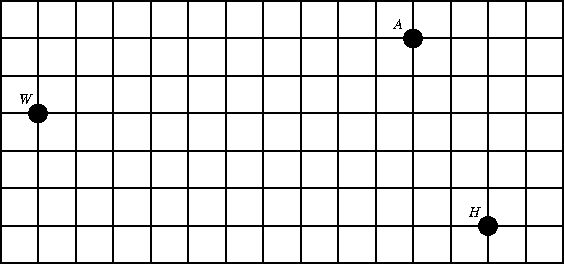
\includegraphics{../graphics/citygrideg2.pdf}
\]
\item Brad and Melissa are going to downtown Champaign, Illinois. Brad
  wants to go to \textit{Jupiter's} for pizza $(J)$ while Melissa goes
  to \textit{Boardman's Art Theater} $(B)$ to watch a movie. Where
  should they park to minimize the total distance walked by both?
  Explain your reasoning.
\[
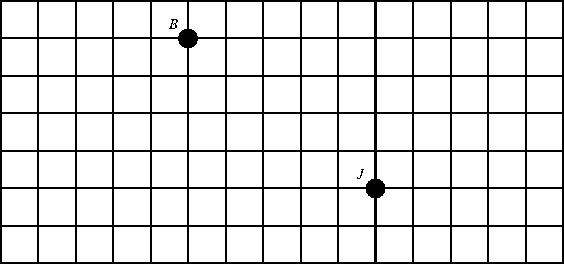
\includegraphics{../graphics/citygrideg3.pdf}
\]

\item Tom is looking for an apartment that is close to Altgeld Hall
  $(H)$ but is also close to his favorite restaurant, \textit{Crane
  Alley}\index{Crane Alley} $(C)$. Where should Tom live? Explain your
  reasoning.
\[
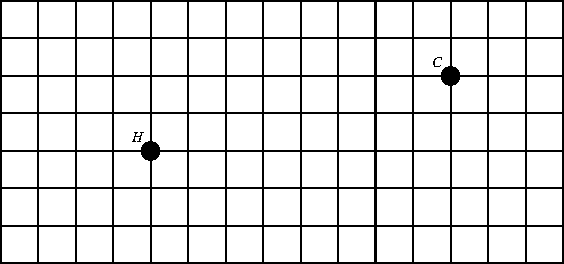
\includegraphics{../graphics/citygrideg6.pdf}
\]


\item Johann and Amber are going to German Village. Johann wants to go
  to \textit{Schmidt's} $(S)$ for a cream-puff while Amber goes to the
  \textit{Thurman Cafe} $(T)$ for some spicy wings. Where should they
  park to minimize the total distance walked by both if Amber insists
  that Johann should not have to walk a longer distance than her?
  Explain your reasoning.
\[
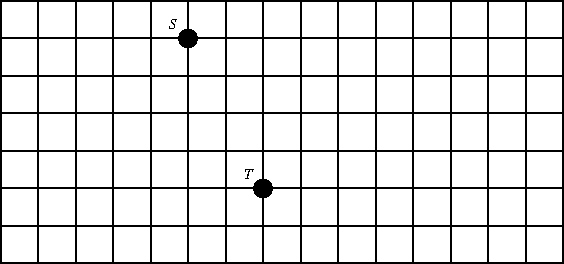
\includegraphics{../graphics/cityST.pdf}
\]

\item Han and Tom are going to downtown Clintonville. Han wants to go
  to get a haircut $(H)$ and Tom wants to look at the bookstore
  $(B)$. Where should they park to keep the total distance walked by
  both less than $8$ blocks? Explain your reasoning.
\[
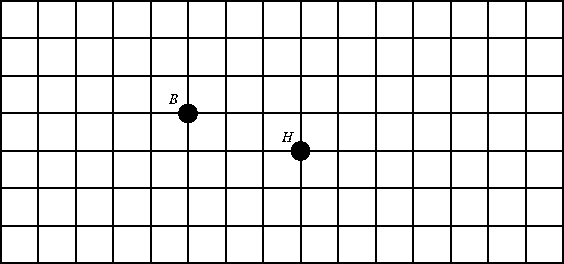
\includegraphics{../graphics/cityBH.pdf}
\]

%\item A group of hooligans think it would be hilarious to place a
%  bucket on the Alma Mater's\marginnote{The Alma Mater is a statue of a
%    ``Loving Mother'' at the University of Illinois.} head, point
%  $A$. Moreover, these hooligans are currently at point $S$ and wish
%  to celebrate their accomplishment at \textit{Murphy's Pub}, point
%  $M$. If there are campus police at points $P$ and $Q$, what path
%  should the hooligans take from $S$ to $A$ to $M$ to best avoid
%  detainment for their hijinks? \index{bucket!Alma Mater} Explain your
%  reasoning.
%\[
%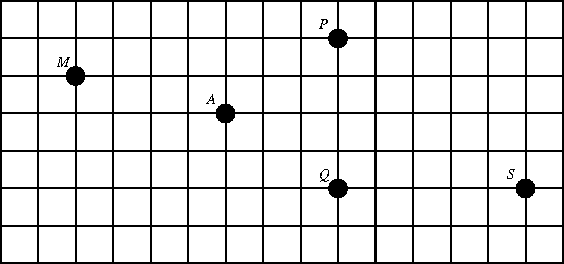
\includegraphics{../graphics/citygrideg8.pdf}
%\]


%\item Scott wants to live within 4 blocks of a cafe $(C)$, within 5
%  blocks of a bar $(B)$, and within 10 blocks of Altgeld Hall,
%  $(A)$. Where should he go apartment hunting? Explain your reasoning.
%\[
%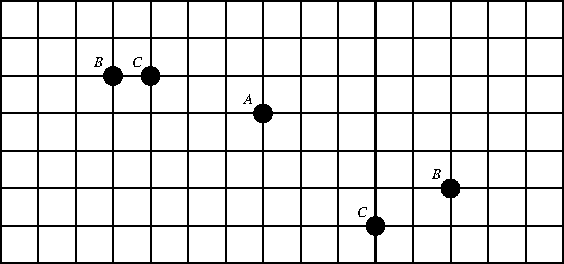
\includegraphics{../graphics/citygrideg9.pdf}
%\]
\item The university is installing emergency phones across
  campus. Where should they place them so that their students are
  never more than a block away from an emergency phone? Explain your
  reasoning.
%%Now compare your answer to the map at
%%http://www.dps.uiuc.edu/ephone/. THIS IS GOOD---BUT WE NEED A GOOD
%%PICT

\item Tom and Ben have devised a ingenious\index{puzzle-stroll}
  \textit{Puzzle-Stroll} (aka a \textit{scavenger-hunt}).
  Here is one of the puzzles:
\begin{quote}
To find what you seek, you must be one with the city---using it's
distance, the treasure is $4$ blocks from $(A)$, $3$ blocks from
$(B)$, and $2$ blocks from $(C)$.
\end{quote}
\[
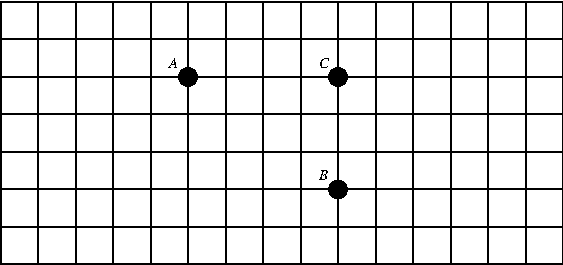
\includegraphics{../graphics/cityPS.pdf}
\]
Where's the treasure? Explain your reasoning.

\item Johann is starting up a new business, \textit{Cafe Battle
  Royale}\index{Battle Royale}. He knows mathematicians drink a lot of
  coffee so he wants it to be near Altgeld Hall. Balancing this
  against how expensive rent is near campus, he decides the cafe
  should be $3$ blocks from Altgeld Hall. Where should his cafe be
  located? Explain your reasoning.


\item \emph{Cafe Battle Royale, Inc}.\ is expanding. Johann wants his
  potential customers to always be within 4 blocks of one of his
  cafes.  Where should his cafes be located? Explain your reasoning.

\item There are hospitals located at $A,B$, and $C$. Ambulances should
  be sent to medical emergencies from whichever hospital is
  closest. Divide the city into regions in a way that will help the
  dispatcher decide which ambulance to send. Explain your reasoning.
\[
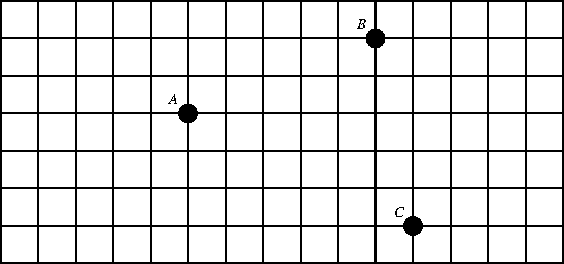
\includegraphics{../graphics/citygrideg10.pdf}
\]

\item Sylvia is going to open a new restaurant called
  \textit{Grillvia's} where customers make their own food and then she
  grills it for them. She wants her restaurant to be equidistant from
  the heart of Champaign $(C)$ and the heart of Urbana $(U)$. Where
  should she put her restaurant?  Explain your reasoning.
\[
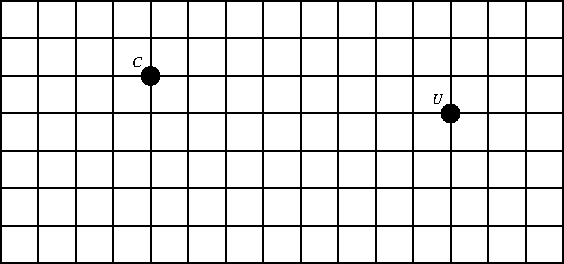
\includegraphics{../graphics/cityGrill.pdf}
\]
\item Chris wants to live an equal distance from his favorite hangout
  \textit{Studio 35} $(S)$ and High Street $(H)$ where he can catch
  the Number 2 bus. Where should he live? Explain your reasoning.
\[
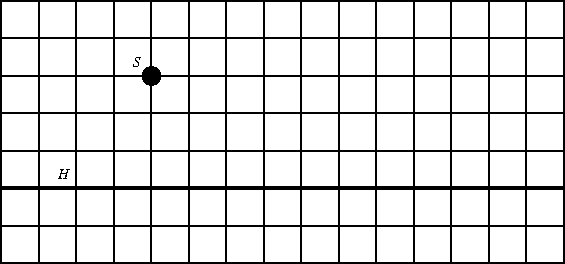
\includegraphics{../graphics/cityHigh.pdf}
\]
%\item Jennifer has just taken a job in Salt Lake City. She wants to
%  live an equal distance from the $228$ bus on Foothill Drive $(F)$
%  and her favorite restaurant, \textit{The Blue Plate Diner}
%  $(B)$. Where should Jennifer dwell? Explain your reasoning.
%\[
%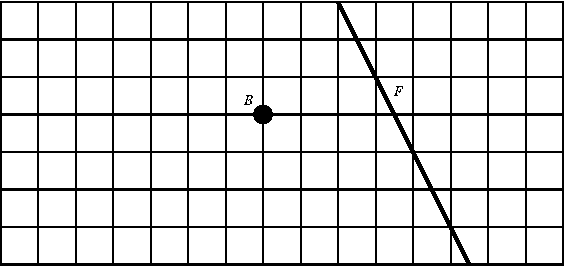
\includegraphics{../graphics/citySalt.pdf}
%\]

\item Lisa just bought a 3-wheeled zebra-striped\index{zebra} electric
  car and its range is limited. Suppose that each day Lisa likes to go
  to work $(W)$, and then to the tea shop $(T)$ \textbf{or} the garden
  shop $(G)$ but not both, and then back home $(H)$. Where should Lisa
  live? Give several options depending on how efficient her
  zebra-striped car is. Explain your reasoning.
\[
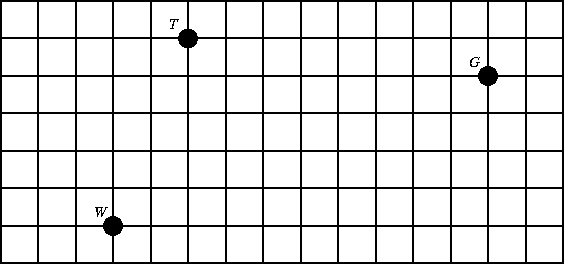
\includegraphics{../graphics/cityZeb.pdf}
\]
\end{enumerate}
\end{problems}
